% ===========================================================================

% ===========================================================================
\documentclass[11pt]{article}
\usepackage[margin=1in,top=1.1in,bottom=1.1in]{geometry}
\usepackage[utf8]{inputenc}
\usepackage[T1]{fontenc}
\usepackage{amsmath,amssymb,amsthm}
\usepackage{graphicx}
\usepackage{booktabs}
\usepackage{array}
\usepackage{makecell}
\usepackage{caption}
\usepackage{float}
\usepackage{placeins}
\usepackage{xcolor}
\usepackage{microtype}
\usepackage{multicol}
\usepackage[colorlinks=true,linkcolor=blue,citecolor=blue,urlcolor=blue]{hyperref}
% Auto-generated by tools/sync_crossrefs.py; do not edit manually.
\makeatletter
\newcommand{\SuppRef}[1]{\csname SuppRef@#1\endcsname}
\expandafter\newcommand\csname SuppRef@eq:supp-axis-agreement\endcsname{S11}
\expandafter\newcommand\csname SuppRef@eq:supp-coherent-response\endcsname{S8}
\expandafter\newcommand\csname SuppRef@eq:supp-conditional-score\endcsname{S14}
\expandafter\newcommand\csname SuppRef@eq:supp-field-decomposition\endcsname{S1}
\expandafter\newcommand\csname SuppRef@eq:supp-joint-spectrum\endcsname{S7}
\expandafter\newcommand\csname SuppRef@eq:supp-local-tensors\endcsname{S9}
\expandafter\newcommand\csname SuppRef@eq:supp-medium-normalization\endcsname{S13}
\expandafter\newcommand\csname SuppRef@eq:supp-nematic\endcsname{S10}
\expandafter\newcommand\csname SuppRef@eq:supp-pd-scores\endcsname{S5}
\expandafter\newcommand\csname SuppRef@eq:supp-phase-centre\endcsname{S3}
\expandafter\newcommand\csname SuppRef@eq:supp-rank-null\endcsname{S6}
\expandafter\newcommand\csname SuppRef@eq:supp-ridge\endcsname{S4}
\expandafter\newcommand\csname SuppRef@eq:supp-road-basis\endcsname{S2}
\expandafter\newcommand\csname SuppRef@fig:supp-1\endcsname{S1}
\expandafter\newcommand\csname SuppRef@fig:supp-2\endcsname{S2}
\expandafter\newcommand\csname SuppRef@fig:supp-3\endcsname{S3}
\expandafter\newcommand\csname SuppRef@fig:supp-4\endcsname{S4}
\expandafter\newcommand\csname SuppRef@fig:supp-5\endcsname{S5}
\expandafter\newcommand\csname SuppRef@fig:supp-6\endcsname{S6}
\expandafter\newcommand\csname SuppRef@fig:supp-7\endcsname{S7}
\expandafter\newcommand\csname SuppRef@note:anisotropy-results\endcsname{S8}
\expandafter\newcommand\csname SuppRef@note:baselines\endcsname{S5}
\expandafter\newcommand\csname SuppRef@note:coupling-results\endcsname{S6}
\expandafter\newcommand\csname SuppRef@note:data\endcsname{S1}
\expandafter\newcommand\csname SuppRef@note:estimation\endcsname{S2}
\expandafter\newcommand\csname SuppRef@note:reproducibility\endcsname{S10}
\expandafter\newcommand\csname SuppRef@note:spatial\endcsname{S4}
\expandafter\newcommand\csname SuppRef@note:spectral\endcsname{S3}
\expandafter\newcommand\csname SuppRef@note:spectral-results\endcsname{S7}
\expandafter\newcommand\csname SuppRef@note:structural-results\endcsname{S9}
\expandafter\newcommand\csname SuppRef@tab:artifact-map\endcsname{S3}
\expandafter\newcommand\csname SuppRef@tab:crosscity\endcsname{S2}
\expandafter\newcommand\csname SuppRef@tab:observation-regimes\endcsname{S1}
\makeatother

\hypersetup{pdftitle={Road-supported effective constitutive coupling and anisotropic routing responses in urban mobility},pdfauthor={Tiehang Xu, Jiahui Wang, Junyan Yang, Qiao Wang},pdfsubject={Urban mobility and constitutive coupling},pdfkeywords={urban mobility, Hodge decomposition, road networks, anisotropy}}
\newcommand{\repositorylocation}{\url{https://github.com/Wangwangw233/paper-urbanflow}}

\captionsetup{font=small,labelfont=bf,width=0.95\textwidth}
\graphicspath{{../../figures/main/}{../../figures/supplementary/}}
\setlength{\emergencystretch}{2em}

% --- notation --------------------------------------------------------------
\newcommand{\R}{\mathbb{R}}
\newcommand{\E}{\mathbb{E}}
\newcommand{\Cov}{\operatorname{Cov}}
\newcommand{\diag}{\operatorname{diag}}
\newcommand{\rank}{\operatorname{rank}}
\newcommand{\tr}{\operatorname{tr}}
\newcommand{\argmin}{\operatorname*{arg\,min}}
\newcommand{\Prj}{P_{\mathrm{r}}}
\newcommand{\Psir}{\Psi_{\mathrm{r}}}
\newcommand{\PsirS}{\Psi_{\mathrm{r},S}}
\newcommand{\GS}{G_{S}}
\newcommand{\DS}{\mathcal{D}_{S}}
\newcommand{\Fcirc}{F^{\circ}}
\newcommand{\Fcond}{F^{\mathrm{cond}}}
\newcommand{\Rcond}{R^{2}_{\mathrm{cond}}}
\newcommand{\Rrouting}{R^{2}_{\mathrm{routing}}}
\newcommand{\Fbar}{\bar{F}_{\phi(t)}}
\newcommand{\xbar}{\bar{x}_{\phi(t)}}
\newcommand{\dx}{\delta x}
\newcommand{\dxt}{\delta x_{t}}
\newcommand{\Aw}{A_{W}}
\newcommand{\Tzero}{T_{0}}
\newcommand{\Gr}{G_{\mathrm{r}}}
\newcommand{\Dr}{D_{\mathrm{r}}}
\newcommand{\T}{\mathsf{T}}
\newcommand{\phim}{\varphi(t)}
\newcommand{\norm}[1]{\lVert #1 \rVert}
\newcommand{\ones}{\mathbf{1}}
\newcommand{\bOne}{b_{1,t}}
\newcommand{\eps}{\varepsilon_{t}}
\newcommand{\Fhat}[1]{\widehat{#1}}
\newcommand{\Rdep}{R^{2}_{\mathrm{dep}}}
\newcommand{\Rclock}{R^{2}_{\mathrm{clock}}}
\newcommand{\UR}{U_{R}}
\newcommand{\deff}{d_{\mathrm{eff}}}
\newcommand{\Efull}{E_{\mathrm{full}}}
\newcommand{\Rr}{\mathcal{R}_{R}}
\newcommand{\CR}{C_{R}}
\newcommand{\Ccal}{\mathcal{C}}
\newcommand{\Px}{P_{x}}
\newcommand{\Ptr}{P_{\mathrm{tr}}}
\newcommand{\Gh}{G_{h}}
\newcommand{\Gl}{g_{\ell}}
\newcommand{\Esh}{E_{\mathrm{shared}}}
\newcommand{\Etem}{E_{\mathrm{tem}}}
\newcommand{\Lcoh}{\Lambda_{h}}
\newcommand{\SigC}{\Sigma_{C}}
\newcommand{\SigU}{\Sigma_{U}}
\newcommand{\AC}{A_{C}}
\newcommand{\AU}{A_{U}}
\newcommand{\Lc}{L_{c}}


\title{Road-supported effective constitutive coupling and anisotropic routing responses in urban mobility}
\author{Tiehang Xu$^{1}$ \and Jiahui Wang$^{2}$ \and Junyan Yang$^{3}$ \and Qiao Wang$^{1,2,\ast}$\\[0.5em]
\small
\begin{tabular}{@{}l@{}}
$^{1}$School of Information Science and Engineering, Southeast University, Nanjing, 210096, China\\
$^{2}$School of Economics and Management, Southeast University, Nanjing, 210096, China\\
$^{3}$School of Architecture, Southeast University, Nanjing, 210096, China\\
Emails: tiehangxu@seu.edu.cn; wangjh0521@seu.edu.cn; yjy-2@163.com; qiaowang@seu.edu.cn\\
$\ast$Correspondence: qiaowang@seu.edu.cn
\end{tabular}
}
\date{}
\begin{document}
\maketitle

\begin{abstract}
Conservation determines where urban movement accumulates and dissipates, but not the routes that carry it. Here we identify an effective linear response linking these two sectors. A Hodge decomposition separates observed flows into source--sink balance and divergence-free routing; we fit the response within a road-supported routing space and evaluate it on held-out dates. The relation captures day-specific routing organization in three cities, strongest in Porto and weakest in Chengdu. The fitted operator exhibits strong local directional selectivity, revealing directional organization beyond a map of roads. The road-supported space is specific against rank-matched random subspaces, while mobility-derived spatial media outperform a road-only medium at equal nominal capacity. Together, these results establish an interpretable effective coupling between source--sink organization and anisotropic routing responses in urban mobility.
\end{abstract}

% Nature Cities Article: introduction without a heading.
\label{sec:intro}
Cities organize movement as well as activities. The location of homes, jobs and services determines where journeys begin and end, while the arrangement of streets shapes the spaces through which those journeys pass. Neighbourhoods with similar net inflows can nevertheless experience different through-movement, and a redistribution of activity need not produce a proportional redistribution of traffic. Gravity, radiation and spatial-interaction models describe flows between places \cite{simini2012universal,lenormand2016systematic,rong2024survey,cabanastirapu2025gravity,simini2021deepgravity}; traffic assignment links demand to routes through travel costs and behavioural rules \cite{wardrop1952,morandi2024assignment}; and graph-based learning offers flexible descriptions of traffic and assignment \cite{wu2019graphwavenet,liu2024endtoend}. Between aggregate interaction and individual routes lies a useful urban-scale object: the local direction and intensity of collective movement.

Field descriptions make this intermediate scale accessible. Recurrent commuting can be represented by a vector field whose potential identifies mobility basins \cite{mazzoli2019field}; trajectory-based formulations extend the approach beyond commuting \cite{liu2024generalized}; and Laplacian evolution identifies urban source--sink patterns \cite{zhang2024laplacian}. Hodge decomposition separates a potential-driven component, associated with the imbalance between arrivals and departures, from circulation that redistributes movement without changing that balance \cite{aoki2022hodge,du2026landscapes}. The two sectors are geometrically orthogonal, but spatial orthogonality does not preclude reproducible statistical coupling. Related field studies identify scaling, temporal response, directional organization and anomalous movement \cite{shida2020scaling,shida2022potential,zhao2024directionality,yang2023vector}. Whether changes in one sector systematically accompany changes in the other is the question that turns a descriptive decomposition into an empirical relation.

We approach this question through an effective constitutive relation: a response connecting the source--sink organization of observed flows to the routing component left undetermined by balance. Roads provide a spatial medium that can be measured independently of the mobility values used to estimate the response \cite{barthelemy2011,kirkley2018,boeing2019,ewing2010travel,sharmin2018}. The operator asks whether a compact linear mapping can reproduce part of the routing organization, and whether that mapping is specific to the road-defined support rather than to any conservation-compatible subspace of the same size.

Here we estimate this response from trajectories in Porto, San Francisco and Chengdu. UrbanFlow constructs a road-supported routing space, fits a linear source--routing operator on training dates and evaluates it on held-out dates. The analysis links three aspects of the same response: its held-out predictive content, its frequency-resolved structure and its local directional organization.

\section{Results}\label{sec:results}
\subsection{Effective response}\label{sec:formulation}

We represent hourly movement as signed crossings of the faces between spatial cells. For a flux field \(F_t\), its discrete divergence \(x_t=DF_t\) records the cellwise source--sink balance. Here \(x_t\) denotes the divergence of the observed coarse-grained flux, not an independently measured origin--destination demand field. The field separates into a minimum-norm component fixed by that balance and a divergence-free routing component,
\begin{equation}\label{eq:f-decomposition}
 F_t=D^\dagger x_t+F_t^\circ,\qquad DF_t^\circ=0.
\end{equation}
Figure~\ref{fig:concept} illustrates the physical freedom: different directional configurations can carry the same source and sink. The two components are spatially orthogonal, but their organization can covary across observations. Predicting the routing component from the source therefore tests a statistical relationship between the irrotational and divergence-free sectors of the measured flow.

\begin{figure}[!t]
\centering
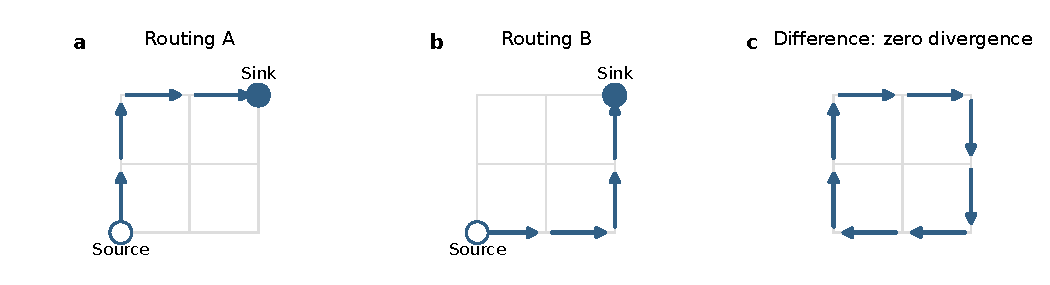
\includegraphics[width=\textwidth]{fig01_concept.pdf}
\caption{\textbf{Routing freedom under conservation.} \textbf{a,b}, Two routes share a source and sink. \textbf{c}, Their difference has zero divergence. Balance fixes the source--sink pattern but leaves routing undetermined.}
\label{fig:concept}
\end{figure}

Road geometry defines an orthonormal basis \(U_R\) within the divergence-free space. The road-coordinate state is \(y_t=U_R^\top F_t^\circ\); a fitted response \(K_R\) relates this state to the source. The corresponding operator in physical space is
\begin{equation}\label{eq:f-reduced}
 \widehat F_t^\circ=C_Rx_t,\qquad C_R=U_RK_RP_x,
\end{equation}
where \(P_x\) restricts inputs to conservation-compatible source patterns. Roads supply the structural support; dated mobility observations determine the response within it. This separation makes the operator interpretable as an effective property of movement in a given urban medium.

The road space captures most of the observed routing energy in Porto and San Francisco and a substantial share in Chengdu (Supplementary Table~\SuppRef{tab:crosscity}). This makes the response interpretable in a spatial medium defined independently of the mobility values used to estimate it.

\subsection{Road-supported coupling}\label{sec:recon}

Operators are estimated on training dates and evaluated on held-out dates. P scores the raw routing field, whereas D tests day-specific departures after removing the training-estimated recurrent hourly pattern (Methods). Figure~\ref{fig:threecity-evidence}a--c shows that the road-supported operator recovers a meaningful share of both components across the three cities. Porto exhibits the strongest departure response; San Francisco retains a clear response; Chengdu is dominated by recurrent daily structure.




\begin{figure}[!t]
\centering
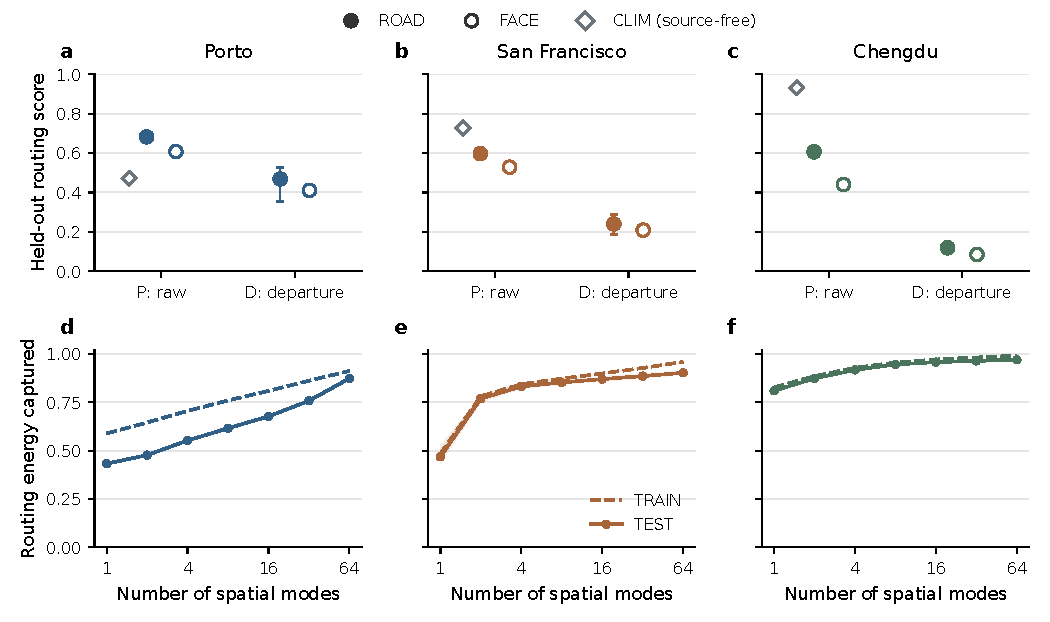
\includegraphics[width=\textwidth]{fig02_threecity_coupling.pdf}
\caption{\textbf{Held-out coupling and spatial organization.} \textbf{a--c}, Raw (P) and departure (D) scores on ROAD (filled) and FACE (open) support, pooling TEST errors; diamonds show the source-free P/ROAD climatology. D/ROAD points carry 95\% paired-date bootstrap intervals. \textbf{d--f}, Energy captured by TRAIN-derived POD modes on TRAIN (dashed) and TEST (solid). San Francisco curves show fold means and ranges. Chengdu uses the 14-date, 06--23\,h window. POD capture measures representation, not source-based prediction.}
\label{fig:threecity-evidence}
\end{figure}

Porto's departure score reaches 0.468 (95\% interval 0.355--0.528), and San Francisco's reaches 0.240 (0.188--0.288). A source--routing pairing null, which permutes complete date blocks and refits the operator, produces no draw approaching either observed score. The full-field gain from the same departures is largest in Porto and much smaller in San Francisco and Chengdu. Exact scores, intervals and Chengdu's descriptive small-sample results are given in Supplementary Note~\SuppRef{note:coupling-results}. Representative physical reconstructions are retained in Supplementary Fig.~\SuppRef{fig:supp-6}.



The spatial modes expose a complementary difference (Fig.~\ref{fig:threecity-evidence}d--f). Chengdu's routing is concentrated in a small number of reproducible modes, whereas Porto's organization is distributed across more modes. A compact spatial representation and a source-based response therefore describe distinct aspects of the field.

Full-face ridge and training-only POD representations outperform the road restriction on the same target (Supplementary Table~\SuppRef{tab:crosscity}). Roads thus provide an interpretable spatial medium rather than an unrestricted approximation of the field.

\subsection{Frequency response}\label{sec:spectra}

The descriptive joint spectra are reported in Supplementary Fig.~\SuppRef{fig:supp-1}. The frozen operator is evaluated frequency by frequency without fitting a new temporal response (Fig.~\ref{fig:threecity-response}). Because prediction and observation are complex Fourier coefficients, we report a phase-sensitive score,
\begin{equation}\label{eq:m-phase-score}
 R_m^2=1-\frac{\sum_d\|a_{d,m}-b_{d,m}\|^2}{\sum_d\|a_{d,m}\|^2},
\end{equation}
and the pooled signed alignment
\begin{equation}\label{eq:m-phase-signed}
 \widetilde\gamma_m=\frac{\sum_d\operatorname{Re}(a_{d,m}^*b_{d,m})}
 {\sqrt{\sum_d\|a_{d,m}\|^2}\sqrt{\sum_d\|b_{d,m}\|^2}},
\end{equation}
where $a_{d,m}$ and $b_{d,m}$ are observed and predicted coefficients on date $d$ (Methods). The response is strongest for the time-independent and low-frequency components, then weakens toward higher harmonics. The phase-sensitive score falls below zero in several bins in San Francisco and Chengdu. The phase-insensitive magnitude $|\gamma_m|$, shown for comparison, can therefore remain high even when the complex response is not reconstructed accurately.

\begin{figure}[!t]
\centering
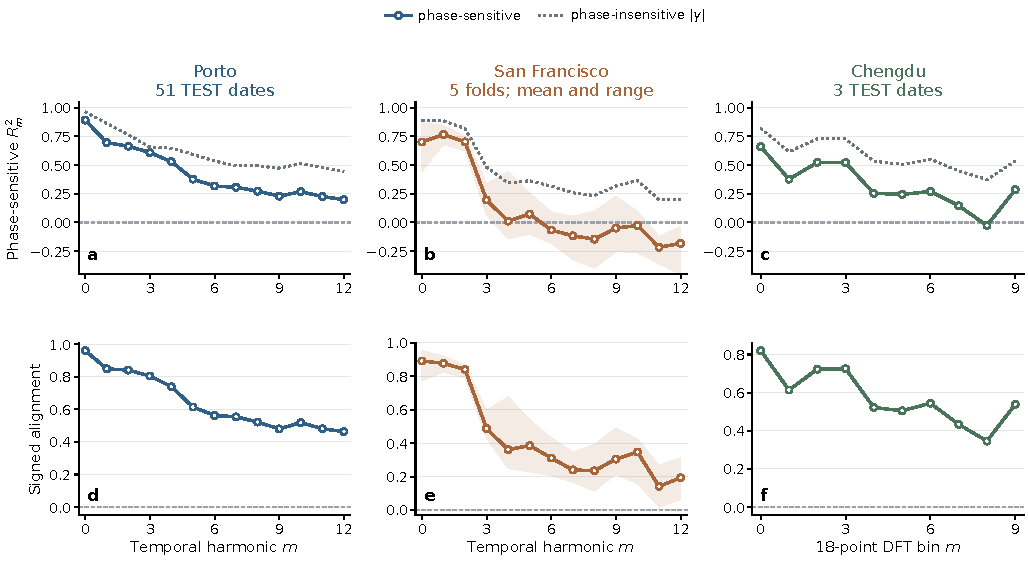
\includegraphics[width=\textwidth]{fig03_frequency_response.pdf}
\caption{\textbf{Frequency-resolved response.} \textbf{a--c}, Per-bin phase-sensitive $R_m^2$ using per-date complex coefficients. \textbf{d--f}, Signed alignment $\widetilde\gamma_m$, which pools date-wise complex inner products. The dotted curve in \textbf{a--c} is the phase-insensitive magnitude $|\gamma_m|$ from TEST-date mean coefficients. The frozen P-selected operator is used throughout. San Francisco shows fold means and ranges. Porto and San Francisco use 24-point DFTs; Chengdu uses all ten bins of its 18-point observed-block DFT.}
\label{fig:threecity-response}
\end{figure}

\subsection{Anisotropy and matched capacity}\label{sec:structure}

The fitted response is strongly anisotropic in every city (Fig.~\ref{fig:road-tests}a--c; full distributions in Supplementary Fig.~\SuppRef{fig:supp-4}). Its local directional selectivity exceeds that of the road-support tensor and varies substantially across space. San Francisco's anisotropy map is stable across date folds. Source-covariance weighting preserves this selectivity, showing that the realized excitation statistics also produce pronounced directional organization. Orientation agreement with the road support is reported in Supplementary Note~\SuppRef{note:anisotropy-results}.

Road geometry also identifies a distinctive routing space. Against 999 rank-matched random subspaces of $\ker D$, every random basis leaves more routing energy uncaptured than the road-induced basis (Fig.~\ref{fig:road-tests}d). The road space is therefore specific within the full aligned observation pool, not merely a convenient choice of coordinates.

At matched nominal capacity, a mobility-inferred medium improves on the road-only medium in every city (Fig.~\ref{fig:road-tests}e). The paired mobility-minus-road differences are positive with narrow date-resampled intervals, while spatial permutation removes the mobility medium's advantage. Road geometry supplies a specific and interpretable support; the learned response additionally contains organization encoded in the mobility data (Supplementary Note~\SuppRef{note:structural-results}).

\begin{figure}[!t]
\centering
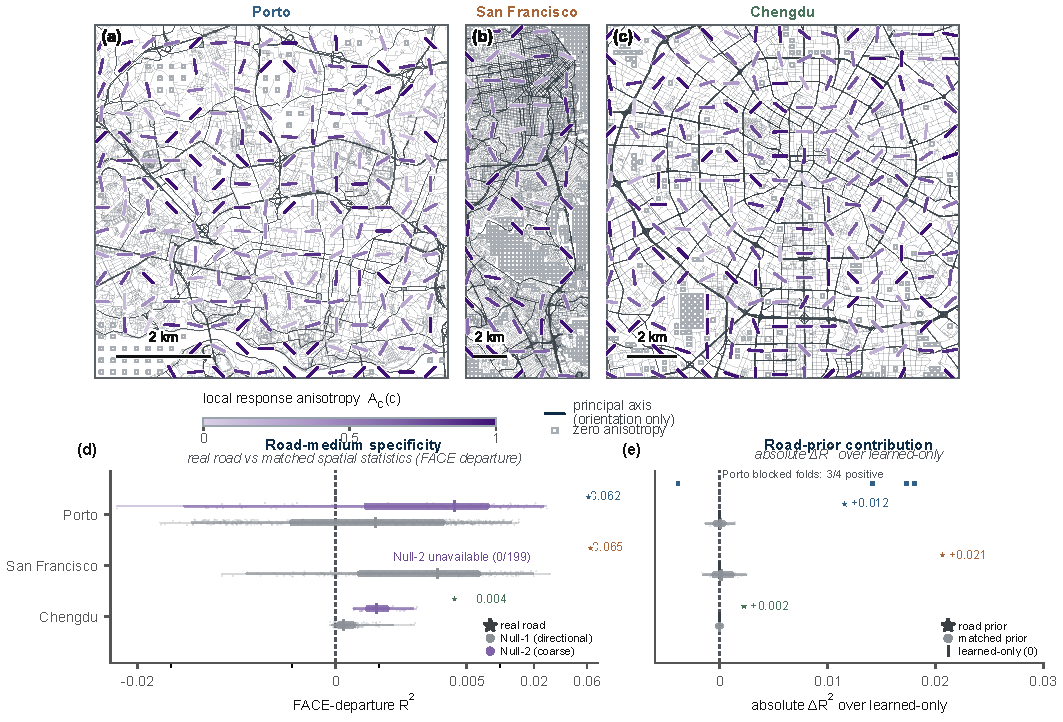
\includegraphics[width=\textwidth]{fig04_anisotropy_road_tests.pdf}
\caption{\textbf{Anisotropy and matched capacity.} \textbf{a--c}, Local response anisotropy $A_C$ on 250\,m regular interior lattices at true aspect (San Francisco: five-fold consensus). Colour shares 0--1; segments show axial directions for $A_C>0.02$ and hollow squares mark zero anisotropy. Streets are \textcopyright~OpenStreetMap contributors. \textbf{d}, Excess unexplained energy $\Delta E$ for 999 rank-matched random subspaces in fixed $\ker D$; the road basis is at zero. Thick/thin marks show 1--99\%/full null ranges. \textbf{e}, Paired mobility-minus-road $\Delta R^2$ at $R=n_{\rm int}$ with 95\% date-resampled intervals. Scores use raw routing against each TEST-date mean; equal $R$ matches nominal capacity, not information. Chengdu's interval is descriptive. Axis agreement is evaluated in Supplementary Note~\SuppRef{note:anisotropy-results}; media are shown in Supplementary Fig.~\SuppRef{fig:supp-5}.}
\label{fig:road-tests}
\end{figure}

\subsection{Model comparison}\label{sec:comparison}

Table~\ref{tab:mainstream-main} compares the source-to-routing operator with unrestricted linear representations and a completed Graph WaveNet adaptation. It also reports the separate OD-estimation and network-loading diagnostics. The inference block uses the same pooled per-date error convention for every row.

Full-face ridge and POD achieve higher reconstruction accuracy, while UrbanFlow exceeds the completed Graph WaveNet adaptation in all three cities under the common pooled convention. The archived Porto paired contrast and sealed-seed robustness are reported in Supplementary Note~\SuppRef{note:baselines}. The loading rows diagnose the implemented demand--registration--loading pipeline; they are not source-only predictions.

\begin{table}[!htbp]
\centering\small
\caption{\textbf{Model comparison.}}
\label{tab:mainstream-main}
\setlength{\tabcolsep}{7pt}
\begin{tabular*}{\textwidth}{@{\extracolsep{\fill}}llrrr@{}}
\toprule
Model & Metric & Porto & San Francisco & Chengdu \\
\midrule
\multicolumn{5}{@{}l}{\emph{Source-to-routing inference}}\\
UrbanFlow & $R_{\rm P,FACE}^2$ & 0.607 & 0.528 & 0.440 \\
Full-face ridge & $R_{\rm P,FACE}^2$ & 0.701 & 0.611 & 0.572 \\
POD regression & $R_{\rm P,FACE}^2$ & 0.701 & 0.637 & 0.575 \\
Graph WaveNet & $R_{\rm P,FACE}^2$ & 0.497 & 0.254 & 0.275 \\
\midrule
\multicolumn{5}{@{}l}{\emph{OD estimation}}\\
Gravity & CPC & 0.525 & 0.464 & 0.555 \\
\midrule
\multicolumn{5}{@{}l}{\emph{Network-loading diagnostics}}\\
Gravity + AON & $R_{\rm FACE}^2$\textsuperscript{a} & 0.136 & 0.270 & $<0.001$ \\
TEST OD + AON & $R_{\rm FACE}^2$\textsuperscript{a} & 0.172 & 0.336 & 0.002 \\
TEST OD + AON & $R_{\rm FACE}^2$\textsuperscript{b} & 0.126 & $-0.533$ & $-0.565$ \\
\bottomrule
\end{tabular*}
\par\smallskip
\parbox{\textwidth}{\footnotesize Inference rows share sources, splits and targets; TEST errors are pooled from per-date numerators and denominators. Gravity uses TRAIN OD margins; AON denotes all-or-nothing assignment. \textsuperscript{a}Amplitude fitted on TEST. \textsuperscript{b}Fixed amplitude, $\alpha=1$. Graph WaveNet reports archived single draws; sealed-seed robustness and the archived Porto paired contrast are in Supplementary Note~\SuppRef{note:baselines}. Loading rows diagnose the implemented pipelines; Chengdu's loading is margin-dominated. Full protocols: Methods and Supplementary Note~\SuppRef{note:reproducibility}.}
\end{table}

The gravity and loading results separate these tasks from source-to-routing inference. Gravity uses TRAIN OD margins; the loading rows additionally use TEST-fitted amplitudes or TEST OD. Chengdu's loading remains largely margin-driven. Detailed protocols are in Supplementary Notes~\SuppRef{note:baselines} and \SuppRef{note:reproducibility}.

\section{Discussion}\label{sec:disc}
\subsection{A constitutive description of urban movement}

The identified operator adds an empirical relation to the Hodge decomposition: source--sink organization and divergence-free routing are orthogonal at one instant, yet covary across observations. This is the constitutive content of UrbanFlow. The response is strongest in Porto, weaker in San Francisco and small in Chengdu, where recurrent structure already accounts for much of the field. The comparison with unrestricted representations further shows that the road-supported object is interpretable rather than merely accurate.

The lifted operator $C_R$ maps a distributed source pattern to a directional routing response. Its columns describe model-implied responses to compatible source directions, while its local tensors expose spatially varying directional selectivity. The phase-sensitive frequency analysis and the anisotropy analysis therefore characterize the same response in time and space. Together, they turn a fitted matrix into an interpretable description of urban movement at the observation scale.

\subsection{Urban anisotropy and the role of roads}

Anisotropy separates the geometry available to movement from the directional response expressed through it. The fitted response is locally selective rather than organized around one city-wide axis. The orientation of these tensors is less informative than their magnitude: axis agreement with road support does not exceed a spectrum-matched rotation null. We therefore interpret anisotropy as a property of the fitted operator on its identified source span, not as independent evidence of road-aligned response. This connects street configuration \cite{hillier1993,penn1998,wang2012} to a measured operator.

Roads play two roles in this framework. As a geometric support, they identify a specific divergence-free space; as a response medium, they do not exhaust the organization encoded in the mobility data. The matched-capacity comparison makes this distinction explicit. A road-only medium is not sufficient, but the road-supported operator remains interpretable and specific. The appropriate conclusion is a road-supported effective coupling, not a road-determined constitutive law.

\subsection{Scope and further tests}

Several boundaries define the next experiments. Signed source balance compresses movement: different OD pairings and opposing flows can produce the same net balance. Chengdu has only three held-out dates in the primary protocol, so its departure interval and pairing null are descriptive; its matched-capacity interval uses four alternate-hour dates. The rank-matched null does not compare rotated or rewired road networks at the same rank, input and target. A decisive structural intervention would make that comparison directly. Nonlinear responses, additional state variables and longer memory are further testable extensions.

The operator is an effective description of the sampled city, not an intervention model. Sources and targets come from the same trajectories, and each city's operator is fitted separately. Forecasting from independently available demand, transfer between cities and model-implied effects of infrastructure changes require further validation. The contribution is a partial, identifiable effective object whose structural support, directional organization and unexplained variation can be measured separately.

\section{Methods}\label{sec:methods}
\subsection{Data and discrete fields}\label{sec:d-data}

Porto uses ECML/PKDD taxi trajectories \cite{ucitaxi2015}: 252 dates, a chronological TRAIN/VAL/TEST split of 151/50/51 dates and a $32\times32$ lattice. San Francisco uses Cabspotting \cite{cabspotting2009}: 15 dates, five blocked folds of 9/3/3 dates and a $32\times88$ lattice. Chengdu uses DiDi ride-hailing trajectories \cite{didi2014chengdu} with 30-second sampled fixes and a $60\times60$ lattice. Its P/D, coherent-response, anisotropy and spectral analyses use a 14-date 8/3/3 subset from the continuous-observation regime. The matched-capacity medium sweep uses a separate chronological 10/4/4 split whose four held-out dates are 26--29 August 2014; these dates belong to the alternate-hour delivery phase, with nine alternating recorded hours per date. The structural null is evaluated on the 19 valid dates of the aligned grid. These protocols are related but not interchangeable. The hourly phase sets are 00--23\,h for Porto/San Francisco and 06--23\,h for Chengdu. Each city is estimated separately. Observation regimes and frozen date lists are specified in Supplementary Note~\SuppRef{note:data} and Supplementary Table~\SuppRef{tab:observation-regimes}.

Successive trajectory segments are walked through the aligned nominal 250\,m cells. Signed crossings of each interior face are accumulated in 60-minute windows to form $F_t\in\mathbb R^{n_f}$. No map matching is applied. For the cell--face incidence matrix $D\in\mathbb R^{n_c\times n_f}$,
\begin{equation}\label{eq:m-project}
 x_t=DF_t,\quad P_0=I-D^\dagger D,\quad F_t^\circ=P_0F_t,
 \quad P_x=DD^\dagger .
\end{equation}
The routing target is calculated from the same crossing field as the source. The Laplacian solve is gauge-pinned. The source is an observed coarse-grained divergence, not an independently measured OD demand field.

The archived footprint mask is the union of cells with non-zero density over all dates, $(\mathrm{N}>0).\mathrm{any}(0)$. It is transductive and is used only for analysis and display; it is not an input to $D$, $U_R$ or $K_R$, which depend on the grid, study domain and road registration.

\subsection{Road space and response estimation}\label{sec:m-cons}

The drivable OpenStreetMap layer \cite{haklay2008} is registered to the study complex. Let $B_R$ be its node--edge incidence, $A_R$ the edge-to-face lift and $\Pi$ the registration map satisfying $DA_R=\Pi B_R$. A cycle basis $Z_R$ satisfies $B_RZ_R=0$. The Gram eigendecomposition of $A_RZ_R$ gives
\begin{equation}\label{eq:m-roadbasis}
 U_R=\operatorname{orth}(A_RZ_R),\qquad U_R^\top U_R=I,
 \qquad DU_R=0,\qquad y_t=U_R^\top F_t^\circ .
\end{equation}
Geometry, study domain and road registration determine $U_R$. Supplementary Note~\SuppRef{note:estimation} gives the registration conventions.

For any source or target $v_t$, TRAIN phase means and departures are
\begin{equation}\label{eq:m-centre}
 \bar v_\phi=\frac{1}{n_{\mathrm{tr},\phi}}
 \sum_{t\in\mathrm{TRAIN}:\phi(t)=\phi}v_t,
 \qquad \delta v_t=v_t-\bar v_{\phi(t)} .
\end{equation}
Stack $\delta x_t^\top$ and $\delta y_t^\top$ as the rows of $X$ and $Z$. Ridge estimation yields
\begin{equation}\label{eq:m-fit}
 \begin{aligned}
 K_R^\star&=\argmin_K\{\|Z-XK^\top\|_F^2+\lambda\|K\|_F^2\}\\
 &=Z^\top X(X^\top X+\lambda I)^{-1},\qquad
 C_R=U_RK_R^\star P_x .
 \end{aligned}
\end{equation}
We use $\lambda=\kappa s_{\max}(XX^\top)$ and select $\kappa$ on VAL from the grid specified in Supplementary Note~\SuppRef{note:estimation}. The archived values are $\kappa=0.01$ in Porto, $0.1$ in San Francisco and $0.1$ in Chengdu's D frame; the Chengdu P-frame sensitivity uses $0.001$. Comparison arms select regularization in the specified scoring frame. Full-face ridge fits $F_t^\circ$ and projects predictions with $P_0$; POD estimates its output basis from TRAIN departures and selects rank and regularization using FACE validation error.

\subsection{Scoring}\label{sec:m-frames}

Define $T_t=U_R^\top F_t^\circ$ on ROAD support and $T_t=F_t^\circ$ on FACE support. Let $B_{\mathrm P}$ and $B_{\mathrm D}$ denote the fitted maps on that support. Both use TRAIN departures; P selects on raw VAL inputs/targets, while D selects on VAL departures using TRAIN means. Predictions have no fitted intercept:
\begin{equation}\label{eq:m-scores}
 \begin{aligned}
 R_{\mathrm P}^2&=1-\frac{\sum_{t\in\mathrm{TEST}}\|T_t-B_{\mathrm P}x_t\|^2}
 {\sum_{t\in\mathrm{TEST}}\|T_t\|^2},\\
 R_{\mathrm D}^2&=1-\frac{\sum_{t\in\mathrm{TEST}}\|\delta T_t-B_{\mathrm D}\delta x_t\|^2}
 {\sum_{t\in\mathrm{TEST}}\|\delta T_t\|^2}.
 \end{aligned}
\end{equation}
Numerators and denominators are pooled across TEST observations and folds within each city. The denominators are target energies. The source-free reference is $\bar T_{\phi(t)}$, reported in Supplementary Table~\SuppRef{tab:crosscity}.

\subsection{Structural tests}

For any orthonormal routing basis $U$, the uncaptured-energy statistic is
\begin{equation}\label{eq:m-null}
 E(U)=1-\frac{\sum_t\|U^\top F_t^\circ\|^2}{\sum_t\|F_t^\circ\|^2},
 \qquad \Delta E_b=E(U_b)-E(U_R).
\end{equation}
Let $K_D$ be an orthonormal basis of $\ker D$. Each null draw uses $G_{ij}\overset{\mathrm{iid}}{\sim}N(0,1)$, $Q=\operatorname{orth}(G)$ and $U_b=K_DQ$ at rank $\operatorname{rank}(U_R)$. The test uses the full aligned observation pool and no source-response fit; this pool differs from the frozen P/D comparison pool.

The second test compares road, mobility-inferred and spatially permuted mobility media at equal nominal block capacity $R$. Each per-face medium is reduced to the same $R$ on nested spatial partitions before mean-1/floor normalization; $R=1$ gives the constant-medium reference. Permutation preserves values, partition and nominal block count. The archived statistic is the equal-date mean of
\begin{equation}\label{eq:m-conditional}
 R_{\mathrm{cond},d}^2=1-
 \frac{\sum_{t\in d}\|T_t-\widehat T_t\|^2}
 {\sum_{t\in d}\|T_t-\langle T\rangle_d\|^2}.
\end{equation}
Figure~\ref{fig:road-tests}e reports the paired-date interval for mobility minus road at $R=n_{\rm int}$, the number of interior faces (1984, 5512 and 7080); Supplementary Fig.~\SuppRef{fig:supp-5} reports each medium's gain over the constant medium. Chengdu uses the archived all-motion channel and a four-date held-out protocol. This date-centred statistic is separate from Eq.~\ref{eq:m-scores}. Source files and partitions are specified in Supplementary Note~\SuppRef{note:spatial}.

\subsection{Anisotropy}

For each regular interior cell, $L_c$ sums signed face flux into two physical components. Define
\begin{equation}\label{eq:m-tensors}
\begin{aligned}
 \Sigma_C(c)&=L_cC_RC_R^\top L_c^\top,\\
 \Sigma_U(c)&=L_cU_RU_R^\top L_c^\top,\\
 A(c)&=\begin{cases}
 (\lambda_1(c)-\lambda_2(c))/(\lambda_1(c)+\lambda_2(c)),&\lambda_1(c)+\lambda_2(c)>0,\\
 0,&\lambda_1(c)+\lambda_2(c)=0 .
 \end{cases}
\end{aligned}
\end{equation}
Here $\lambda_1\geq\lambda_2$ are the eigenvalues of the relevant tensor. The principal eigenvector defines an axial orientation $\theta$ modulo $\pi$. San Francisco uses the per-cell mean anisotropy and nematic mean orientation over five folds. We also evaluate the source-covariance-weighted response tensor
\begin{equation}\label{eq:m-response-tensor}
 \Sigma_{\rm response}(c)=L_cC_R\Sigma_{xx}C_R^\top L_c^\top,
\end{equation}
with $\Sigma_{xx}$ the TRAIN covariance of source departures. Structural-axis agreement is evaluated on regular interior cells for which both anisotropies are nonzero, using the frozen joint-anisotropy weighting
\begin{equation}\label{eq:axis-agreement}
 G_{\theta}=\frac{\sum_c A_C(c)A_U(c)\cos[2(\theta_C(c)-\theta_U(c))]}
 {\sum_c A_C(c)A_U(c)} .
\end{equation}
To test whether this agreement exceeds what the shared road subspace and operator spectrum imply, write $K_R=Q\Lambda V^\top$ and replace $Q$ by a Haar-random orthonormal frame $Q_0$ in the road output space, $K_0=Q_0\Lambda V^\top$. We recompute $G_\theta$ for 999 draws.

Only regular interior cells enter the anisotropy statistics; their metric $L_cL_c^\top=2I$ is isotropic. Metric and rotation checks are specified in Supplementary Note~\SuppRef{note:spatial}.

\subsection{Spectra and coherent response}

For the joint spectrum in Supplementary Fig.~\SuppRef{fig:supp-1}, each TRAIN date is transformed separately, retaining its mean. For field $v_{d,j}$ and observed block length $N$,
\begin{equation}\label{eq:m-spectrum}
 \begin{aligned}
 Z_{d,m}&=N^{-1/2}\sum_{j=0}^{N-1}v_{d,j}e^{-2\pi imj/N},\qquad f_m=m/N,\\
 P_m&=w_m\langle\|Z_{d,m}\|^2\rangle_d,\qquad
 J_{m,k}=\frac{P_m}{\sum_lP_l}\frac{s_{m,k}^2}{\sum_a s_{m,a}^2}.
 \end{aligned}
\end{equation}
$s_{m,k}$ are singular values of the date-by-space coefficient matrix. The weights are $w_0=w_{N/2}=1$ and $w_m=2$ otherwise. Porto/San Francisco use $N=24$; Chengdu uses $N=18$ with no night-time imputation. Frequencies are cycles per observed hour. San Francisco averages $P_m$ and within-frequency mode shares separately across folds before multiplication. The first eight modes are displayed after full-spectrum normalization. Spatial POD curves in Fig.~\ref{fig:threecity-evidence} use a raw TRAIN routing basis.

For the frequency-resolved response, each TEST date is transformed with the same unitary DFT used for the descriptive spectrum: 24 points in Porto/San Francisco and 18 points in Chengdu. Let $a_{d,m}$ and $b_{d,m}$ be the observed and predicted road-coordinate coefficients on date $d$ at bin $m$. We report
\begin{equation}\label{eq:m-coherent}
 R_m^2=1-\frac{\sum_d\|a_{d,m}-b_{d,m}\|^2}{\sum_d\|a_{d,m}\|^2},
 \qquad
 \widetilde\gamma_m=\frac{\sum_d\operatorname{Re}(a_{d,m}^*b_{d,m})}
 {\sqrt{\sum_d\|a_{d,m}\|^2}\sqrt{\sum_d\|b_{d,m}\|^2}},
\end{equation}
where the signed alignment pools date-wise complex inner products and energies across TEST dates. The phase-insensitive magnitude $|\gamma_m|=|a_m^*b_m|/(\|a_m\|\|b_m\|)$ uses TEST-date mean coefficients and is reported for comparison. The P-selected operator is fixed. All ten single-sided bins are evaluated in Chengdu.

\subsection{Baselines and uncertainty}

Graph WaveNet uses the frozen splits, a 300-epoch budget and a four-point VAL-selected grid, with phase-centred TRAIN data and raw VAL/TEST data (P/FACE). Table~\ref{tab:mainstream-main} uses archived pooled per-date errors; sealed seed robustness and the archived Porto paired contrast are reported in Supplementary Note~\SuppRef{note:baselines}. Graphormer's reduced-budget run is excluded. Configurations and outputs are indexed in Supplementary Note~\SuppRef{note:reproducibility}.

Gravity estimates OD flows from TRAIN margins and distance, selecting friction on VAL. Its overlap is $\mathrm{CPC}=2\sum_{ij}\min(\widehat Q_{ij},Q_{ij})/(\sum_{ij}\widehat Q_{ij}+\sum_{ij}Q_{ij})$ at $4\times4$-cell aggregation. AON uses time-shortest paths, road costs and a 150\,m snap threshold; gravity loading retains the top 150,000 zone pairs. Scaled diagnostics fit $\alpha^*$ on TEST; the fixed-amplitude arm uses $\alpha=1$. Chengdu OD uses maximal occupied runs under the frozen cleaning rules. Registration and loading conventions are specified in Supplementary Note~\SuppRef{note:baselines}; no radiation or user-equilibrium score is estimated.

Primary D intervals use 10,000 resamples of held-out dates within each fold and the 2.5/97.5 percentiles; faces are never resampled. The source--routing pairing null permutes complete date blocks within TRAIN, VAL and TEST separately and refits the operator in each of 199 draws. Neural contrasts use 9,999 date resamples with Holm adjustment within city/support; matched-capacity contrasts use 10,000 paired-date resamples. Structural nulls use 999 draws. Chengdu's pairing null is descriptive because it has only three held-out dates; its equal-capacity interval resamples four dates.

\section*{Data availability}
Porto and San Francisco use the cited public datasets; Chengdu uses the archived DiDi ride-hailing sample \cite{didi2014chengdu}. Data versions and checksums are recorded in the repository data manifest. Road data derive from OpenStreetMap and retain the OpenStreetMap contributors attribution. Frozen splits and observation regimes are tabulated in the supplementary material. The public export contains no individual-level trajectory records; redistribution status and any external-data requirements for derived fields are recorded in its data manifest.
\section*{Code availability}
The analysis repository separates figure rebuilding from frozen products, core-score recomputation and end-to-end raw-trajectory reconstruction. The matched-capacity modules, phase-sensitive frequency metrics, anisotropy rotation null and figure generators are included. The matched-capacity sweep still requires external aligned fields, date-freeze files and GIS rasters, which are listed with hashes in the data manifest; no raw trajectories are included. Large prediction files and original training artifacts that are not in the export are identified rather than represented as included. Execution requirements and checksums are documented in the repository manifest. Public repository location: \repositorylocation.

% Reference list: compact spacing keeps the bibliography from leaving a
% short trailing page without changing the body text layout.
{\scriptsize\makeatletter\def\@listi{\leftmargin\leftmargini \parsep 0\p@ \topsep 2\p@ \itemsep 0\p@}\let\@listI\@listi\makeatother
\begin{multicols}{2}
\bibliographystyle{unsrt}
\bibliography{refs}
\end{multicols}
}
\end{document}
